\subsection{Halfspaces}
\label{sec:halfspaces}
We will introduce hyperplanes and halfspaces and talk about their geometric properties. We will see that they are convex and have rather strong intersection properties. Later, we will introduce strongly separated halfspaces, whose special role will become apparent in Section~\ref{sec:group}. Lastly, we will be concerned with some combinatorial properties of halfspaces. The first part of this section follows particularly closely the lecture notes by \textcite{Rolli2012}.

\begin{defin}[Hyperplanes]
  Let \(X\) be a cube complex
  \begin{itemize}
  \item 0-, 1- and 2-dimensional cubes are respectively called \emph{vertices, edges and squares}.
  \item A \emph{square relation} on the set of edges is given by \(e \sim e'\) if and only if there is a sequence of edges \(e_1, \dots, e_n\), such that \(e_1 = e\) and \(e_n = e'\) and such that any two edges \(e_{i-1}, e_i\) are opposite edges in a common square in \(X\). If we allow for an edge to be opposite to itself, this yields an equivalence relation of the set of all edges.
  \item A midcube \(M \subset X\) is \emph{transverse} to a square relation class \(E = [e]_\sim\), write \(M \pitchfork E\), if \(M \cap X^{(1)}\) contains only midpoints of edges in \(E\).
  \item The \emph{hyperplane} defined by \(E\) is given by
    \begin{align*}
      \mathfrak{\hat h}(E) \coloneqq \bigcup_{M \pitchfork E} M \subset X.
    \end{align*}
    If the equivalence class \(E\) is not important, we will often write \(\mathfrak{\hat h}\) instead of \(\mathfrak{\hat h}(E)\).
  \end{itemize}
\end{defin}

\begin{bsp}
  Figure~\ref{fig:hyperplanes} contains an example of a CAT(0) cube complex with an edge equivalence class of edges (dark blue) and associated hyperplane (light blue). 
  \begin{figure}[htbp]
    \centering
    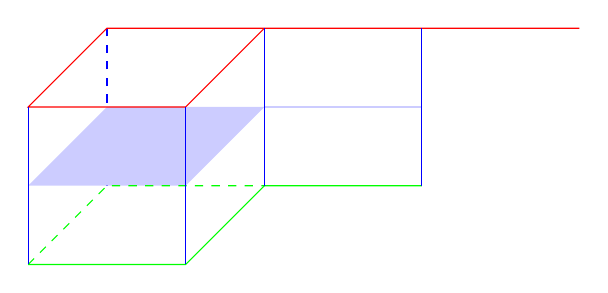
\begin{tikzpicture}
  [scale=2]
  \draw[blue,dashed] (0.5,0.5) -- (0.5,1.5);
  \fill[blue!20] (0, 0.5) -- (1, 0.5) -- (1.5, 1) -- (0.5, 1) -- (0, 0.5);
  \draw[blue!20] (1.5,1) -- (2.5,1);
  \draw[red] (1.5, 1.5) -- (1,1) -- (0,1) -- (0.5,1.5) -- (1.5,1.5) -- (2.5,1.5)  -- (3.5,1.5);
  \draw[green] (2.5,0.5) -- (1.5,0.5) -- (1,0) -- (0,0);
  \draw[green,dashed] (0,0) -- (0.5,0.5) -- (1.5,0.5);
  \draw[blue] (0,0) -- (0, 1)
  (1,0) -- (1,1)
  (1.5,0.5) -- (1.5,1.5)
  (2.5,0.5) -- (2.5,1.5);
\end{tikzpicture}

%%% Local Variables:
%%% mode: latex
%%% TeX-master: "../Master"
%%% End:

    \caption{Example of a CAT(0) cube complex with a hyperplane inscribed. The dark blue edges form an edge equivalence class, which defines the blue hyperplane. The red and green parts indicate the two halfspaces associated to the hyperplane. The figure follows closely the example in \textcite{sageev-lecture-notes}.}
    \label{fig:hyperplanes}
  \end{figure}
\end{bsp}

\begin{prop}[Convexity of halfspaces,{\cite[Propositions 18 \& 19]{Rolli2012}}]
  Let \(X\) be a CAT(0) cube complex and \(\mathfrak{\hat h} \subset X\) be a hyperplane. Then \(\mathfrak{\hat h}\) is closed and convex. Furthermore, if \(\mathfrak{\hat h}\) contains at least two points of the image of any geodesic \(\gamma\), then the whole image of \(\gamma\) is contained in \(\halfspace{\hat h}\).
\end{prop}

\begin{cor}
  Let \(X\) be a CAT(0) cube complex. Every \(\mathfrak{\hat h} \subset X\) is itself a CAT(0) cube complex.
\end{cor}

\begin{thm}[Separation, {\cite[Proposition 21]{Rolli2012}}]
  Any hyperplane \(\mathfrak{\hat h}\) separates \(X\) in exactly two convex connected components.
\end{thm}

\begin{defin}[Halfspaces]
  The two connected components of \(X \setminus \mathfrak{h}\) are called \emph{halfspaces}. If \(\halfspace{h} \subset X \setminus \mathfrak{\hat h}\) is one of these halfspaces, then \(\halfspace{h}^\ast\) denotes the opposite halfspace leading to \(X = \halfspace{h}\, \sqcup\, \mathfrak{\hat h}\, \sqcup\, \halfspace{h}^\ast \).
\end{defin}

\begin{bsp}
  Figure~\ref{fig:hyperplanes} also indicates the two halfspaces (red and green color).
\end{bsp}

\begin{thm}[Intersection, {\cite[Proposition 22 \& 24]{Rolli2012}}]
  \label{thm:common-intersection}
  \begin{enumerate}
  \item Let \(\mathfrak{h}_1, \dots, \mathfrak{h}_n\) be halfplanes with pairwise non-trivial intersection. Then
    \begin{align*}
      \bigcap_{i=1}^n \mathfrak{h}_i \neq \varnothing.
    \end{align*}
  \item Let \(\halfspace{h}_1, \dots, \halfspace{h}_n\) be halfspaces with pairwise non-trivial intersection. Then
    \begin{align*}
      \bigcap_{i=1}^n \halfspace{h}_i \neq \varnothing.
    \end{align*}
    In particular, the intersection contains a vertex of \(X\).
  \end{enumerate}
\end{thm}

This closes our discussion of geometric properties. The following definition will play a central role in Section~\ref{sec:group} (see for example Proposition~\ref{prop:cs-5.1}).

\begin{defin}[Strongly separated halfspaces]
  \label{defin:strong-sep}
  Two parallel hyperplanes are called \emph{strongly separated} if there is no hyperplane transverse to both. Two halfspaces are called \emph{strongly separated} if the same is true for their associated hyperplanes.
\end{defin}

We close this section with two technical results. The first is concerned with the countability of \(\mathcal{H}\) which is an important technical detail for the metrizability of the Roller compactification (see Corollary~\ref{cor:comp-met}). The second result shows is the last missing step to see that every CAT(0) cube complex gives rise to a discrete pocset as defined in the next section.

\begin{cor}
  \label{cor:halfspace-countable}
  If \(X\) is a locally countable CAT(0) cube complex. Then its set of hyperplanes \(\mathcal{\hat H}\) and its set of halfspaces \(\mathcal{H}\) are countable.
\end{cor}

\begin{proof}
  We fix a vertex \(x_0 \in V(X)\) and consider the sets
  \[
    Y_n \coloneqq \{(x,y) \in X_{n-1} \times X_{n} \mid y \in N(x)\} \subset X_{n-1} \times X_n \quad \forall n \in \N.
  \]
  By Lemma~\ref{lem:lf-countable} the sets \(X_n\) are countable and we have that
  \[
    \mathcal{\hat H} = \bigcup_{n=1}^\infty \bigcup_{e \in Y_n} \mathfrak{\hat h}([e])
  \]
  is countable. Since every hyperplane has exactly two halfspaces associated to it the same is true for \(\mathcal{H}\).
\end{proof}


\begin{lemma}
  \label{lem:finite-interval}
  Let \(X\) be a connected CAT(0) cube complex. Then for any two \(\mathfrak{h,k} \in \mathcal{H}(X)\) such that \(\mathfrak{h} \subset \mathfrak{k}\) we have
  \[
    |\{\mathfrak{l} \in \mathcal{H}(X) \mid \mathfrak{h} \subset \mathfrak{l} \subset \mathfrak{k}\}| < \infty.
  \]
\end{lemma}

\begin{proof}
  We will call the set of the lemma \(M\) and the corresponding set of hyperplanes \(\hat M\). Clearly, the two sets are one-to-one. We take any vertex \(v \in \mathfrak{h}\)  and \(w \in \mathfrak{k}^\ast\). Then there exists a finite edge path \(c\) joining the two. We claim that \(\hat M\) is a subset of all the hyperplanes defined by the edges in \(c\). Indeed, let \(\mathfrak{l} \in M\). Then \(v \in \mathfrak{l}\) and \(w \in \mathfrak{l}^\ast\). Hence, \(c\) has to transverse \(\mathfrak{\hat l}\) meaning that \(\mathfrak{\hat l}\) is one of the hyperplanes defined by an edge in \(c\).
\end{proof}

%%% Local Variables:
%%% mode: latex
%%% TeX-master: "../Master"
%%% End:
